% Revised analysis: selected-reference normalization; see wid_supplement.tex and revision record.
% Empirical values/tables are generated by make_revision_paper.py and make_fusion_robustness_paper.py.
\documentclass[5p,times,twocolumn,final,numbers,sort&compress]{elsarticle}
\usepackage[T1]{fontenc}
\usepackage{amsmath,amssymb,booktabs,tabularx,microtype,graphicx,xcolor}
\usepackage{xurl}
\usepackage[hidelinks]{hyperref}
\usepackage[font=footnotesize,labelfont=rm,skip=3pt]{caption}
\journal{Pattern Recognition Letters}
\hypersetup{pdftitle={Handedness for Bangla writer identification: Oracle gains and predicted-attribute utility},pdfauthor={Tanzim Hasan Prappo; M. Shahidur Rahman}}
% Generated from revised results.
\newcommand{\rWriters}{42}
\newcommand{\rLeft}{21}
\newcommand{\rImages}{336}
\newcommand{\rUnits}{5040}
\newcommand{\rInvalid}{39}
\newcommand{\rSettings}{120}
\newcommand{\rHandShared}{68.7}
\newcommand{\rHandOwn}{65.5}
\newcommand{\rHandWriter}{73.8}
\newcommand{\rLawN}{456}
\newcommand{\rLawR}{0.996}
\newcommand{\rLawMae}{1.5}
\newcommand{\rLawBias}{-0.9}
\newcommand{\rThresholdMed}{86}
\newcommand{\rThresholdMin}{55}
\newcommand{\rThresholdMax}{98}
\newcommand{\rKnownGain}{6.1}
\newcommand{\rKnownLo}{+5.1}
\newcommand{\rKnownHi}{+7.1}
\newcommand{\rFusionGain}{-0.6}
\newcommand{\rFusionLo}{-2.3}
\newcommand{\rFusionHi}{+0.9}
\newcommand{\rFilterGain}{-14.3}
\newcommand{\rFilterLo}{-19.3}
\newcommand{\rFilterHi}{-9.5}
\newcommand{\rLeakEn}{82.1}
\newcommand{\rLeakRandomMin}{52.4}
\newcommand{\rLeakRandomMax}{76.2}
\newcommand{\rBrierOwn}{0.204}
\newcommand{\rNllOwn}{0.602}
\newcommand{\rOracleVsRandom}{-0.8}
\newcommand{\rOracleVsRandomLo}{-1.8}
\newcommand{\rOracleVsRandomHi}{+0.2}
\newcommand{\rRandomKnownGain}{6.9}
\newcommand{\rBothGain}{+1.08}
\newcommand{\rBothLo}{+0.50}
\newcommand{\rBothHi}{+1.72}
\newcommand{\rExampleProduct}{31.4}
\newcommand{\rExampleFilter}{28.0}
\newcommand{\rExampleCondCorrect}{42.7}
\newcommand{\rExampleCondWrong}{58.0}

% Generated by code/make_fusion_robustness_paper.py
\newcommand{\rNestedGain}{-0.08}
\newcommand{\rNestedLo}{-1.13}
\newcommand{\rNestedHi}{+0.81}
\newcommand{\rNestedVsFixedGain}{+0.49}
\newcommand{\rNestedVsFixedLo}{-0.15}
\newcommand{\rNestedVsFixedHi}{+1.28}
\newcommand{\rNestedNllGain}{-0.010}
\newcommand{\rNestedNllLo}{-0.041}
\newcommand{\rNestedNllHi}{+0.024}
\newcommand{\rWeightMedian}{0.5}
\newcommand{\rWeightZero}{1.3}
\newcommand{\rTempLower}{0.8}
\newcommand{\rTempUpper}{2.6}
\newcommand{\rTempNearMedian}{1}
\newcommand{\rSeedAccuracyMin}{64.3}
\newcommand{\rSeedAccuracyMax}{66.7}
\newcommand{\rSeedDisagree}{2.4}
\newcommand{\rSeedGainMin}{-0.57}
\newcommand{\rSeedGainMax}{-0.50}
\newcommand{\rFixedOmitMin}{-0.76}
\newcommand{\rFixedOmitMax}{+0.01}
\newcommand{\rNestedOmitMin}{-0.24}
\newcommand{\rNestedOmitMax}{+0.22}
\newcommand{\rKnownOmitMin}{+5.91}
\newcommand{\rKnownOmitMax}{+6.26}
\newcommand{\rFilterOmitMin}{-14.77}
\newcommand{\rFilterOmitMax}{-13.10}
\newcommand{\rTempGainMin}{-1.81}
\newcommand{\rTempGainMax}{+0.04}

% Generated by code/make_representation_utility.py
\newcommand{\rRepNestedMin}{-0.64}
\newcommand{\rRepNestedMax}{+0.42}
\newcommand{\rRepCorrectionMin}{+0.18}
\newcommand{\rRepCorrectionMax}{+1.08}

% Generated by code/run_margin_diagnostic.py
\newcommand{\rFixedRescued}{2.02}
\newcommand{\rFixedDamaged}{2.59}
\newcommand{\rNestedRescued}{1.33}
\newcommand{\rNestedDamaged}{1.42}

\AtBeginEnvironment{thebibliography}{\interlinepenalty=10000}
\setlength{\textfloatsep}{8pt plus 2pt minus 2pt}
\setlength{\floatsep}{7pt plus 2pt minus 2pt}
\setlength{\dbltextfloatsep}{8pt plus 2pt minus 2pt}
\begin{document}
\begin{frontmatter}
\title{Handedness for Bangla writer identification: Oracle gains and predicted-attribute utility}
\author[sust]{Tanzim Hasan Prappo\corref{cor}}
\ead{2021331006@student.sust.edu}
\author[sust]{M. Shahidur Rahman}
\ead{rahmanms@sust.edu}
\cortext[cor]{Corresponding author.}
\affiliation[sust]{organization={Department of Computer Science and Engineering, Shahjalal University of Science and Technology},city={Sylhet},postcode={3114},country={Bangladesh}}
\begin{abstract}
Attribute-classification accuracy can misrepresent the identification value of a soft biometric. We present a controlled framework separating oracle gains, prediction errors, evidence dependence and writer-associated information, and apply it to BanglaHand: \rWriters{} writers, six representations and \rSettings{} identification settings. Normalization uses selected gallery references only; query-handedness models exclude the queried writer from training and calibration. Known handedness improves top-1 accuracy by \rKnownGain{} percentage points, compared with \rRandomKnownGain{} points for an expected known random partition. With query handedness predicted at \rHandOwn\% accuracy on self-chosen paragraphs, calibrated fixed-weight fusion changes identification accuracy by \rFusionGain{} points, properly nested learned weighting by \rNestedGain{}, and hard filtering by \rFilterGain{}. Neither fusion rule establishes a gain in the designated comparisons. Filtering and margin diagnostics explain how joint correctness and confidence affect ranking. Random writer labels expose writer-associated information in enrolled-writer attribute evaluation. Robustness analyses characterize sensitivity within this cohort. The framework provides reusable controls for evaluating auxiliary attributes in biometric candidate ranking, helping researchers distinguish oracle opportunity from operational benefit and make fusion decisions using measured identification utility.
\end{abstract}
\begin{keyword}
Writer identification \sep Soft biometrics \sep Handedness \sep Bangla handwriting \sep Score fusion \sep Evaluation protocol
\end{keyword}
\end{frontmatter}

\section{Introduction}
A soft biometric describes a person without uniquely identifying them. Gender, age and handedness can supplement identity matching by changing candidate scores or restricting a gallery \cite{jain2004soft,dantcheva2016soft}. Handwriting studies have predicted such attributes from static images \cite{liwicki2011gender,siddiqi2015gender,bouadjenek2016soft,almaadeed2016handedness,morera2018handedness,rahmanian2021handedness}. The downstream question is different: does the predicted attribute improve identification of the writer?

Two issues complicate this question. First, an incorrect hard attribute decision can exclude the true writer. Its utility depends on identification performance conditional on attribute correctness, not just the marginal accuracy of each system. Soft fusion avoids automatic exclusion, but depends on probability calibration and on whether the attribute scores add information to the identity scores. Both can come from the same image and contain redundant evidence. Second, handwriting carries writer-associated information \cite{bulacu2007text,schomaker2007codebooks}. An attribute predictor evaluated on previously seen writers can exploit that information. Such evaluation may match an enrolment-conditioned application, but does not estimate attribute generalization to unseen writers \cite{kaufman2012leakage}.

The contribution of this study is a controlled framework for evaluating whether predicted soft-biometric information provides downstream identification utility. Separating oracle gains, prediction errors, evidence dependence and writer-associated information shows why attribute-classification accuracy alone can be misleading. Known random partitions benchmark oracle opportunity; calibrated fixed and nested learned-weight fusion measure achieved utility; and joint-correctness, margin and random-label diagnostics distinguish sources of apparent gains. The elementary filtering identity and standard fusion rules are diagnostic tools and comparators.

Building on the companion study \cite{prappo2026handedness}, which examines handedness classification and photometric cues, we reuse BanglaHand \cite{banglahand2026data}, its preprocessing, descriptors and frozen network representations. The present study evaluates whether predicted handedness provides downstream writer-identification utility. Its methodological contribution is a controlled evaluation that separates oracle gains from operational gains through random-partition controls, nested fusion-weight selection, and analyses of error dependence and writer-associated information.

\section{Related work}
Handwriting-based attribute studies include gender prediction from online and offline information \cite{liwicki2011gender,siddiqi2015gender}, the ICDAR gender competition \cite{hassaine2013icdar}, and multiple soft traits \cite{bouadjenek2016soft}. Al-Maadeed et al.\ evaluated handedness on Arabic and English handwriting from 121 writers \cite{almaadeed2016handedness}. Morera et al.\ separated training and test individuals when predicting handedness using CNNs \cite{morera2018handedness}; their unbalanced-class overall accuracy is not directly comparable to accuracy on a balanced collection. Rahmanian and Shayegan also reported high handedness accuracy \cite{rahmanian2021handedness}. Differences in class balance, evaluation unit and writer separation limit numerical comparisons across these studies; downstream identification utility must be evaluated separately.

The companion's 77.4\% balanced accuracy aggregates SVM margins over six shared paragraphs under repeated five-fold writer-disjoint evaluation \cite{prappo2026handedness}. Our calibrated single-query probabilities modify identity ranking under leave-one-writer-out fitting; these endpoints are not numerically interchangeable.

Text-independent writer identification uses, among other representations, contour directions, hinges and allographic features \cite{bulacu2007text}, or contour-fragment codebooks \cite{schomaker2007codebooks}. Bangla resources include BanglaWriting \cite{mridha2021banglawriting} and the Boise State collection \cite{majid2018bangla}; Bangla writer verification has also been studied \cite{paul2024bangla}. These tasks and their accuracies are distinct from attribute-assisted closed-set identification. The present study measures the change in identification accuracy when handedness evidence is supplied under explicitly defined query and gallery conditions.

\section{Data and evaluation protocol}
\label{sec:protocol}
\subsection{Queries, references and representations}
BanglaHand contains \rImages{} paragraph photographs from \rWriters{} writers (\rLeft{} left-handed), with common materials and one controlled photographic session \cite{banglahand2026data}. Each writer supplied six shared prompts and two self-chosen texts. A query is a whole paragraph or one of 2, 4 or 8 horizontal strips, approximately 3.5, 1.75 or 0.9 lines. Strip boundaries follow low-ink rows near equally spaced cuts. Of \rUnits{} candidate units, \rInvalid{} fail the fixed feature-validity rules; exclusion counts and weighting are reported in the supplement.

The six representations are STROKE (208 contour and skeleton features), HC-183 (183 ink-mask features), frozen ImageNet ResNet-18, EfficientNet-B0 and ViT-B/16 embeddings \cite{he2016resnet,tan2019efficientnet,dosovitskiy2021vit}, and Stroke-CNN (the same frozen ResNet-18 applied to binary ink tiles). No network is trained on these writers. The supplement specifies mask thresholds, scales, tiles, descriptor components and checkpoints without requiring a companion manuscript.

Identification is closed-set over all writers. A shared-prompt query is compared with the other five prompts of every writer. Self-chosen-text queries are compared with every subset of $k=1,2,3$ or 6 shared reference paragraphs. For each reference configuration, feature means and standard deviations are fitted \emph{only to its selected whole-paragraph gallery references}. The resulting transform is applied to references and queries. Each transformed vector is $L_2$-normalized; a gallery template is the normalized mean of that writer's reference vectors. Cosine similarity $s_w$ supplies the baseline ranking. Query pages and unused reference pages do not fit this transform. Four query sizes, five reference conditions and six representations give \rSettings{} settings.

\subsection{Handedness prediction and score fusion}
For each query writer and unit size, a linear SVM ($C=0.1$) is trained on valid shared units of the other 41 writers using HC-183. Standardization is fitted within training data. Five-fold stratified group cross-validation over those training writers supplies out-of-fold scores for logistic calibration \cite{platt1999probabilistic}. The outer writer's samples and labels are excluded from both stages. Let $p_q=\sigma(\ell_q)$ be the resulting left-hand probability. Adjusted HC-183 and STROKE predictors provide sensitivity checks.

These are cross-validated performance estimates. Writer identity assigns evaluation folds; it is not an input available to a deployed predictor. Deployment would freeze one attribute model and its calibration, temperature and fusion weight using separate development writers, then score every future query without choosing a model by its unknown identity. Training on the enrolled writers instead defines a different target. We do not estimate performance of one universal deployed predictor here.

In the \emph{known} scenario, both query and gallery hands are supplied. This oracle restricts the top-ranked group to the query's true hand. In the primary \emph{predicted-query} scenario, gallery hands are known, and $p_q$ is predicted. Probabilistic score fusion ranks writers by
\begin{equation}
 f_w=s_w/T+\log p_q(h_w),
 \label{eq:fusion}
\end{equation}
where $p_q(1)=p_q$ and $p_q(0)=1-p_q$. For each setting, $T$ is selected from 31 logarithmically spaced values between $10^{-3}$ and 1 by minimizing identification negative log loss on the other query writers, with equal writer weights. Temperature fitting uses identity scores and writer targets, not attribute scores or the held-out query writer's outcomes. Gallery references remain available because this is closed-set identification.

Equation~\eqref{eq:fusion} is a score-combination rule. It has a Bayesian interpretation only under additional assumptions about the dependence of its evidence and the calibration prior. We do not assume these hold for two representations of the same handwriting. Hard filtering instead ranks all writers with the predicted hand ahead of the other hand, preserving identity-score order within each group. In this balanced gallery, an incorrect hand prediction makes top-1 success impossible.

\subsection{Nested fusion-weight comparison}
\label{sec:nested}
We additionally rank candidates by $s_w/T+\lambda\log p_q(h_w)$, selecting a nonnegative weight for each held-out query writer. The other 41 writers supply five development folds, regenerating attribute probabilities inside the outer exclusion to avoid selection bias \cite{cawley2010selection}. Each development attribute model and its inner five-fold writer-group calibrator exclude both the outer writer and the entire development fold. Equal-writer development negative log loss selects $\lambda\in\{0,.1,.2,.3,.5,.7,1,1.5,2,3,5\}$ at the same ID-only temperature as fixed fusion. Final query predictions use the outer model trained on the other 41 writers. The grid includes no attribute evidence ($\lambda=0$) and the fixed rule ($\lambda=1$); exact ties select the smaller weight. Known gallery metadata remain available in development and evaluation. The supplement distinguishes this nested comparison from the historical, incompletely nested weight fit.

\subsection{Filtering identity and controls}
\label{sec:identity}
Let $C$ denote correct attribute prediction and $K$ successful identification with the true query hand supplied. With both groups nonempty, filtered success is $C\cap K$. Thus
\begin{align}
 A_{\mathrm{filter}}&=aP(K\mid C)\nonumber\\
 &=aA_{\mathrm{known}}+\operatorname{Cov}(\mathbf1_C,\mathbf1_K),
 \label{eq:exact}
\end{align}
where $a=P(C)$. Only if the two correctness events are independent does this reduce to
\begin{equation}
 \begin{aligned}
 A_{\mathrm{filter}}&\approx aA_{\mathrm{known}},\\
 a_{\mathrm{break}}&\approx A_{\mathrm{none}}/A_{\mathrm{known}}.
 \end{aligned}
 \label{eq:approx}
\end{equation}
We measure the conditional accuracies and approximation residuals rather than treating the product as universal. The two marginal accuracies alone permit the bounds
\begin{equation}
 \begin{aligned}
 \max(0,a+A_{\mathrm{known}}-1)&\leq A_{\mathrm{filter}},\\
 A_{\mathrm{filter}}&\leq\min(a,A_{\mathrm{known}}).
 \end{aligned}
 \label{eq:bounds}
\end{equation}

Known balanced random writer partitions test how much oracle benefit comes from supplying an arbitrary correct partition. Separately, 20 nearly hand-balanced random 21/21 writer labelings test whether an attribute model can predict arbitrary writer-associated labels. For each labeling, the positive group contains 10 or 11 of the 21 left-handed writers. Writer-held-out prediction is compared with enrolment-trained prediction, where other paragraphs of the same writer are available. The latter is an explicitly different generalization target; it is not a causal decomposition of genuine handedness accuracy.

\subsection{Endpoints and inferential scope}
\label{sec:statistics}
Top-1 accuracy is averaged over valid query units and reference configurations within each writer, then equally over writers. Across-setting means give each of the \rSettings{} settings equal weight. Paired differences use 9,999 writer-level sign flips and 95\% intervals from 10,000 hand-stratified writer bootstraps. The same sampled writer indices are used across settings for aggregate intervals, preserving their dependence. These intervals condition on the observed gallery and fitted predictions; they do not include new-gallery sampling or full model-refitting uncertainty.

Four designated comparisons retain the original study's focus: ResNet-18 and ViT-B/16 on self-chosen paragraphs with one reference and quarter strips with six references. Holm correction covers these four comparisons. They are retrospective evaluation contrasts, not preregistered confirmation: a feasibility analysis had already inspected paragraph-level conditions, and the present normalization correction followed review. The new learned-weight comparisons against no fusion and fixed fusion form eight exploratory contrasts (four settings, two comparators), with Holm correction across all eight. Other robustness analyses are descriptive. No equivalence margin was specified, so nonsignificance is not interpreted as absence of a useful effect.

\section{Results}
\subsection{Known and predicted query handedness}
The primary predictor attains \rHandShared\% accuracy on shared paragraphs and \rHandOwn\% on self-chosen paragraphs; averaging paragraph log-odds within a writer gives \rHandWriter\% over all eight paragraphs. The latter uses more writing and is not the accuracy available for a single query. Sensitivity predictors and strip accuracies appear in the supplement. For self-chosen paragraphs, the primary predictor has Brier score \rBrierOwn{} and negative log loss \rNllOwn{}; the reliability plots and intervals do not isolate miscalibration as the cause of fusion failure.

Known handedness improves top-1 accuracy by \rKnownGain{} percentage points on average (95\% conditional interval [\rKnownLo, \rKnownHi]). Probabilistic score fusion changes it by \rFusionGain{} points [\rFusionLo, \rFusionHi], and hard filtering by \rFilterGain{} points [\rFilterLo, \rFilterHi]. Table~\ref{tab:main} shows two representative reference conditions. Differences between representations are substantial, so an across-setting mean should not be interpreted as the expected accuracy of an arbitrary deployed system. Figure~\ref{fig:performance} shows the effects of query size and reference count.

\begin{table*}[t]
\caption{Top-1 identification accuracy (\%), equally weighted by writer. Known: query and gallery hands supplied. Fusion and Filter: query hand predicted using writer-held-out HC-183; gallery hands supplied. For $k=1$, all six reference choices are averaged within writer.}
\label{tab:main}
\centering\small
\setlength{\tabcolsep}{5pt}
\begin{tabular}{lrrrrrrrr}
\toprule
 & \multicolumn{4}{c}{Self-chosen paragraph, $k=1$} & \multicolumn{4}{c}{Self-chosen quarter strip, $k=6$}\\
\cmidrule(lr){2-5}\cmidrule(lr){6-9}
Representation & None & Known & Fusion & Filter & None & Known & Fusion & Filter\\
\midrule
% Generated by code/make_revision_paper.py; do not edit.
STROKE & 92.3 & 95.4 & 93.3 & 62.3 & 89.0 & 91.1 & 88.7 & 60.0 \\
HC-183 & 39.7 & 48.0 & 37.9 & 28.0 & 33.0 & 42.9 & 32.1 & 25.6 \\
ResNet-18 & 62.9 & 67.9 & 62.1 & 42.3 & 47.4 & 51.7 & 46.0 & 35.8 \\
EffNet-B0 & 51.4 & 60.3 & 51.0 & 36.7 & 49.2 & 57.6 & 48.9 & 38.2 \\
ViT-B/16 & 68.1 & 73.8 & 68.3 & 45.8 & 48.3 & 57.1 & 48.0 & 39.1 \\
Stroke-CNN & 58.7 & 70.8 & 59.9 & 43.8 & 10.7 & 15.5 & 10.7 & 8.3 \\
\bottomrule

\end{tabular}
\end{table*}

\begin{figure*}[t]
\centering
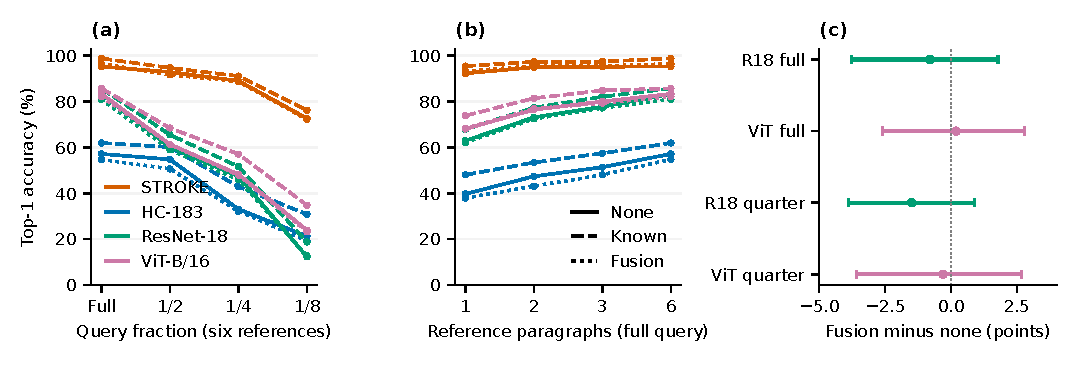
\includegraphics[width=\textwidth]{figures_revision/performance.pdf}
\caption{Identification accuracy for self-chosen texts. (a) Query size with six whole-paragraph references per writer. (b) Reference count for paragraph queries. Solid: no handedness; dashed: known query and gallery hands; dotted: probabilistic fusion with predicted query handedness. (c) Writer-level paired differences for the four designated comparisons, with 95\% conditional bootstrap intervals. Representations omitted from (a,b) remain in the full numerical results.}
\label{fig:performance}
\end{figure*}

Neither fixed nor nested learned weighting establishes a gain in the designated comparisons (Table~\ref{tab:tests}). Across all settings, nested weighting changes top-1 by \rNestedGain{} points [\rNestedLo, \rNestedHi], and differs from fixed weighting by \rNestedVsFixedGain{} points [\rNestedVsFixedLo, \rNestedVsFixedHi]. The median selected weight is \rWeightMedian{}; \rWeightZero\% of outer-writer/setting fits choose zero. This comparison permits downweighting redundant evidence without selecting a weight on the scored writer. It does not exclude small improvements or establish that other fusion families cannot help.

\begin{table*}[t]
\caption{Four designated settings: fixed and nested learned-weight fusion. Entries are paired top-1 differences in percentage points with conditional 95\% writer-bootstrap intervals. Fixed and Nested refer to differences from no fusion. Holm columns adjust the eight new learned-rule comparisons (four settings, two comparators). All comparisons are exploratory.}
\label{tab:tests}
\centering\footnotesize
\setlength{\tabcolsep}{3pt}
\begin{tabular}{llrrrcc}
\toprule
 & & & & & \multicolumn{2}{c}{Holm $p$, Nested vs}\\
\cmidrule(lr){6-7}
Self-chosen query & Representation & Fixed [95\% CI] & Nested [95\% CI] & Nested $-$ Fixed [95\% CI] & None & Fixed\\
\midrule
% Generated by code/make_revision_paper.py; do not edit.
Paragraph, $k=1$ & ResNet-18 & -0.79 [-3.77, +1.79] & -0.20 [-2.18, +1.59] & +0.60 [-0.99, +2.38] & 1.000 & 1.000 \\
Paragraph, $k=1$ & ViT-B/16 & +0.20 [-2.58, +2.78] & +1.19 [-0.40, +2.78] & +0.99 [-0.60, +2.78] & 1.000 & 1.000 \\
Quarter, $k=6$ & ResNet-18 & -1.49 [-3.87, +0.89] & -0.89 [-2.68, +0.89] & +0.60 [-1.49, +2.98] & 1.000 & 1.000 \\
Quarter, $k=6$ & ViT-B/16 & -0.30 [-3.57, +2.68] & -0.30 [-2.98, +1.79] & +0.00 [-1.49, +1.19] & 1.000 & 1.000 \\
\bottomrule

\end{tabular}
\end{table*}

\subsection{Representation-specific utility}
Figure~\ref{fig:representation} compares writer-level means over the 20 settings per representation. Nested-fusion changes range from \rRepNestedMin{} to \rRepNestedMax{} points, and its correction relative to fixed fusion from \rRepCorrectionMin{} to \rRepCorrectionMax{} points. The overall mean conceals differences in oracle opportunity and prediction costs. These marginal exploratory intervals condition on the fitted gallery and predictions; they do not justify selecting a winning representation after inspection.

\begin{figure*}[t]
\centering
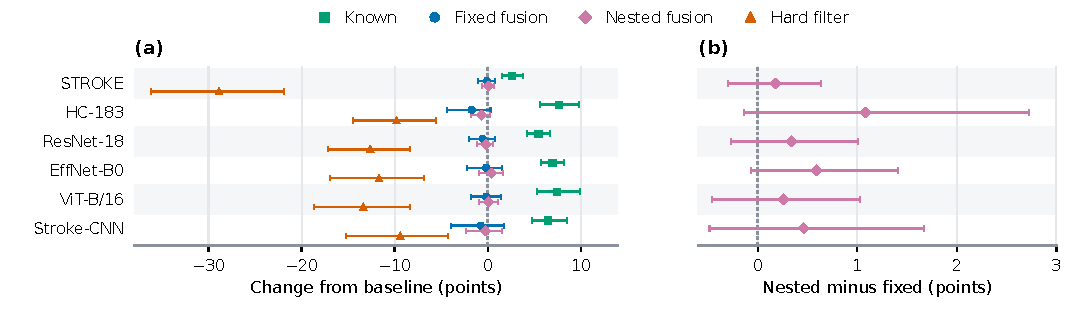
\includegraphics[width=\textwidth]{figures_revision/representation_utility.pdf}
\caption{Representation-specific utility, averaging 20 settings and all 42 writers equally. (a) Top-1 changes from identification without handedness. (b) Nested minus fixed fusion on a separate scale. Bars are marginal conditional 95\% writer-bootstrap intervals with shared resampling across contrasts, not simultaneous confidence bands.}
\label{fig:representation}
\end{figure*}

\subsection{Within-cohort robustness}
Across four grouped calibration partitions, handedness accuracy on self-chosen paragraphs ranges from \rSeedAccuracyMin\% to \rSeedAccuracyMax\%; \rSeedDisagree\% of these queries change predicted hand at least once. Mean gains from fixed fusion range from \rSeedGainMin{} to \rSeedGainMax{} points. Temperature selection reaches the lower grid endpoint in \rTempLower\% and the upper endpoint in \rTempUpper\% of fits. Halving or doubling the selected temperatures gives mean fusion changes from \rTempGainMin{} to \rTempGainMax{} points. Omitting each writer from class-balanced evaluation averaging yields mean changes under nested fusion ranging from \rNestedOmitMin{} to \rNestedOmitMax{} points, while hard filtering remains substantially harmful. The supplement reports loss profiles, paired intervals and every writer's influence. These diagnostics retain the observed gallery and do not constitute independent-dataset validation.

\subsection{Conditional filtering utility}
Across \rLawN{} combinations of setting and prediction model, the independence product tracks filtering accuracy ($r=\rLawR$), with mean absolute error \rLawMae{} points and signed bias \rLawBias{} points. These combinations reuse writers and are not independent replications. The residual analyses in Fig.~\ref{fig:diagnostics} and supplementary conditional accuracies show why the exact identity in Eq.~\eqref{eq:exact} is preferable when predictions are available. For HC-183 identification on self-chosen paragraphs with one reference, the product predicts \rExampleProduct\% versus \rExampleFilter\% observed. Known-hand identification succeeds on \rExampleCondCorrect\% of queries with correct hand predictions and \rExampleCondWrong\% with incorrect predictions. Agreement over a broad performance range can therefore conceal decision-relevant residuals.

For self-chosen queries, the approximate break-even accuracy has median \rThresholdMed\% and range \rThresholdMin--\rThresholdMax\%. This is a property of the tested identifiers and reference conditions under Eq.~\eqref{eq:approx}, not a general handedness requirement. A stronger baseline leaves less room for an imperfect filter to help. A known balanced random partition improves accuracy by \rRandomKnownGain{} points on average. Known handedness differs from that expectation by \rOracleVsRandom{} points (95\% conditional interval [\rOracleVsRandomLo, \rOracleVsRandomHi]). Thus the oracle benefit is consistent with useful partition information, without a distinctive advantage over the random-partition benchmark.

\begin{figure*}[t]
\centering
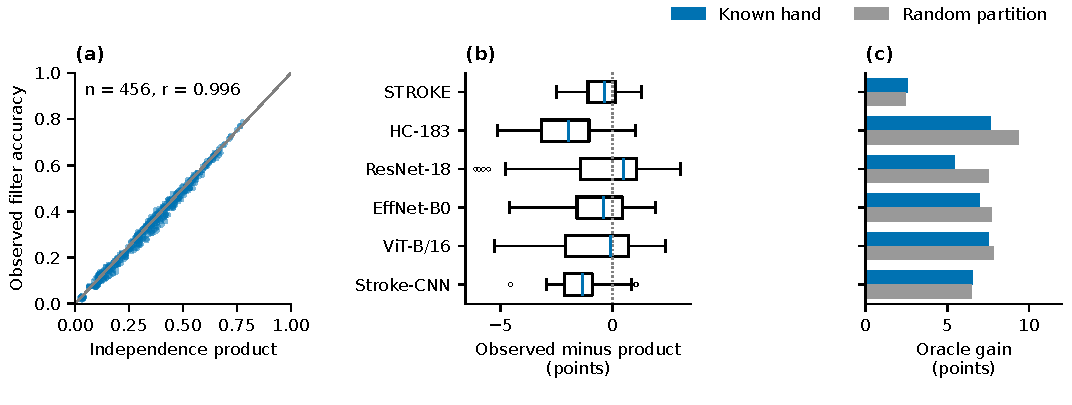
\includegraphics[width=\textwidth]{figures_revision/diagnostics.pdf}
\caption{Filtering diagnostics. (a) Observed filtering accuracy versus the independence product for all evaluated combinations; the line indicates equality. (b) Signed approximation residuals by representation, exposing discrepancies hidden by pooled correlation. (c) Known-handedness gain versus the expected gain of a known balanced random writer partition. These are descriptive comparisons on the observed cohort, not independent dataset replications.}
\label{fig:diagnostics}
\end{figure*}

\subsection{Writer-associated information and exploratory extensions}
With enrolment training, paragraph handedness accuracy on self-chosen texts is \rLeakEn\%, compared with \rHandOwn\% for held-out writers. Under enrolment training, the random-label accuracies range from \rLeakRandomMin\% to \rLeakRandomMax\%. This demonstrates that writer-associated information can support arbitrary labels. It diagnoses a change in the learning problem under writer overlap; it does not demonstrate leakage in the primary writer-held-out pipeline, quantify an identity contribution to genuine handedness accuracy, or rule out acquisition signals. Fixed balanced labels and leave-one-writer-out training also create a structured null; the full random-label distributions are reported without treating a nominal 50\% reference as an exact null distribution.

Exploratory both-sided descriptor agreement improves top-1 by \rBothGain{} points [\rBothLo, \rBothHi] over the 96 self-chosen-text settings (Supplement S6). It replaces known gallery-hand labels with predicted reference descriptors and changes the score rule. An impostor reference model can include the query writer's enrolment pages, so this enrolled-cohort diagnostic does not establish unseen-cohort handedness utility or contradict the primary protocol. Shared-text queries are excluded because those query pages enter impostor-model fitting. Synthetic and reduced-gallery sensitivities remain conditional on their stated models and this cohort.

\section{Discussion}
The methodological lesson is that oracle gains and attribute accuracy do not establish downstream identification utility. Correct metadata reveal an opportunity to improve ranking; an attribute predictor must still supply useful evidence at the decisions where it matters. In this cohort, neither calibrated fixed fusion nor properly nested learned weighting establishes a gain in the designated comparisons. The random-partition benchmark further shows that the oracle advantage is consistent with correct binary partition information, without a distinctive handedness advantage. Hard filtering turns an incorrect hand prediction into an unrecoverable top-1 error. Soft fusion avoids that veto, but calibration alone cannot ensure that overlapping evidence will improve the identity ranking.

The practical criterion also involves identity margins. Fusion preserves ranking within a hand group. Let $m_q=(s_{w^*}-\max_{h_w\ne h_{w^*}}s_w)/T$ and $r_q=\log[p_q(h_{w^*})/p_q(1-h_{w^*})]$. Away from score ties, identification succeeds exactly when the true writer leads its hand group and $m_q+\lambda r_q>0$. True identity enters only this retrospective diagnostic. Attribute accuracy alone therefore omits whether confidence crosses the relevant identity margin. Across settings, fixed fusion rescues \rFixedRescued\% of decisions but damages \rFixedDamaged\%; nested weighting reduces these to \rNestedRescued\% and \rNestedDamaged\%. The supplement gives the decision-level reconstruction, paired intervals and margin plot.

Predictable handedness \cite{prappo2026handedness} is compatible with these outcomes: attribute errors can erase oracle gains, and attribute cues may duplicate identity evidence. Our fusion results do not imply that handedness is unidentifiable.

Nested weighting reduces the mean loss relative to fixed fusion. Since the weight minimizes development log loss, this result concerns that explicit selection objective rather than an exhaustive search for top-1-optimal fusion. The study does not identify a universal attribute-accuracy threshold for soft fusion. The filtering identity serves as a diagnostic of the joint correctness distribution; its product approximation requires independence. Even equal marginal accuracies need not imply equal utility. Likewise, high attribute accuracy on enrolled writers may be appropriate for a declared closed-set application, while overstating performance on unseen writers. The random-label control diagnoses this distinction without assigning a causal fraction to identity.

\subsection{Scope and limitations}
BanglaHand provides a deliberately balanced cohort of \rLeft{} left- and \rLeft{} right-handed writers under controlled acquisition \cite{banglahand2026data}. Recruiting the left-handed group required substantial effort; this balance enables comparisons without majority-class dominance. The estimates describe this \rWriters{}-writer closed gallery from one region, device and photographic session. Broader transfer requires other writers and acquisition conditions; the companion study shares this cohort and is not independent validation. Each writer contributes two self-chosen paragraphs, and strips vary text quantity without adding independent writers.

The uncertainty analyses characterize internal stability conditional on the enrolled gallery and fitted predictions. They do not propagate new-gallery, new-session or full-pipeline-refitting variability. Repeated calibration partitions vary one fitting stage; writer omission changes evaluation averaging while retaining the gallery. These distinctions specify which sources of variation future replication should assess.

The computational comparison uses handcrafted descriptors and frozen ImageNet representations, allowing reproducible evaluation without task-specific network training. Handwriting-specialized training, fine-tuning, stronger identifiers and alternative fusion objectives remain outside this comparison; their different error patterns or margins could change fusion utility. Handedness is the sole real auxiliary attribute tested. BDSHWA records handedness for Bengali--English online handwriting but includes one left-handed participant \cite{bdshwa2026}, so it cannot supply a balanced offline replication.

The primary predicted-query protocol assumes reliable gallery handedness. Knowing a suspect's handedness does not establish the hand of the questioned writer. The known scenario assumes both are reliably available. Closed-set top-1 ranking does not evaluate open-set rejection, evidential likelihood ratios, disguised writing, or non-dominant-hand writing. Application to forensic candidate prioritization would require validation under those operational conditions and explicit treatment of uncertain attributes and error costs. Predicted handedness alone cannot justify exclusion.

\section{Conclusion}
The controlled comparisons show why oracle gains and attribute accuracy cannot substitute for measured identification utility. On this Bangla collection, correct query and gallery handedness improves writer ranking, whereas fixed and properly nested learned-weight fusion of the tested query predictor produce no reliably demonstrated gain over identification alone, and hard filtering causes substantial losses. The analytical filtering diagnostic connects success to joint correctness, while the oracle, predicted-attribute and random-label controls distinguish different sources of apparent utility. Random-label prediction shows that enrolled-writer attribute accuracy can contain substantial writer-associated information. Independent and cross-session studies can assess transfer to other populations and acquisition conditions. Future fusion methods should be evaluated on downstream utility, calibration and error dependence, with the query/gallery information available at deployment stated explicitly.

\section*{Data and code availability}
Code, frozen features, setting manifests, numerical results and self-contained supplementary methods are archived as \href{https://github.com/LegendaryBeast/Bangla-writer-identification-research/releases/download/v1.6.0/wid-reproducibility-v1.6.0.zip}{reproducibility ZIP v1.6.0} at \url{https://github.com/LegendaryBeast/Bangla-writer-identification-research/releases/tag/v1.6.0}. The release supplies exact checkpoint references and table/figure reproduction commands. Code is MIT licensed; results and frozen features are CC BY 4.0. Photographs are excluded; obtain BanglaHand separately from Mendeley Data (doi:10.17632/n4sjstdzfy.1) \cite{banglahand2026data}.

\par\vspace{8pt}
\noindent\begin{minipage}{\columnwidth}
\section*{CRediT authorship contribution statement}
Tanzim Hasan Prappo: Conceptualization, Methodology, Software, Validation, Writing -- original draft, Writing -- review \& editing. M. Shahidur Rahman: Supervision, Writing -- review \& editing.
\par
\end{minipage}

\section*{Ethics, funding and competing interests}
Informed consent was obtained voluntarily before data collection. Handwriting samples use pseudonymous writer identifiers. Writers received an honorarium paid by the authors from personal funds. This research received no specific grant. The authors declare no competing interests.

\section*{Declaration of generative AI use}
An AI assistant was used to audit analysis code, and assist with drafting. The authors are responsible for verifying the analyses, references and final text, and for all publication claims.

\bibliographystyle{elsarticle-num}
\bibliography{references}
\end{document}
